\documentclass[11pt]{article}

\usepackage{tikz}
\usetikzlibrary{calc,patterns,decorations.pathmorphing,decorations.markings}
\usetikzlibrary{intersections}
\usepackage{circuitikz}
\usepackage{amsmath}
\usepackage{amssymb}
\usepackage{float}
\DeclareMathOperator{\Tr}{Tr}

\usepackage{color}
\usepackage{listings}
\usepackage{setspace}
\definecolor{Code}{rgb}{0,0,0}
\definecolor{Decorators}{rgb}{0.5,0.5,0.5}
\definecolor{Numbers}{rgb}{0.5,0,0}
\definecolor{MatchingBrackets}{rgb}{0.25,0.5,0.5}
\definecolor{Keywords}{rgb}{0,0,1}
\definecolor{self}{rgb}{0,0,0}
\definecolor{Strings}{rgb}{0,0.63,0}
\definecolor{Comments}{rgb}{0,0.63,1}
\definecolor{Backquotes}{rgb}{0,0,0}
\definecolor{Classname}{rgb}{0,0,0}
\definecolor{FunctionName}{rgb}{0,0,0}
\definecolor{Operators}{rgb}{0,0,0}
\definecolor{Background}{rgb}{0.98,0.98,0.98}
\lstdefinelanguage{Python}{
numbers=left,
numberstyle=\footnotesize,
numbersep=1em,
xleftmargin=1em,
framextopmargin=2em,
framexbottommargin=2em,
showspaces=false,
showtabs=false,
showstringspaces=false,
frame=l,
tabsize=4,
% Basic
basicstyle=\ttfamily\small\setstretch{1},
backgroundcolor=\color{Background},
% Comments
commentstyle=\color{Comments}\slshape,
% Strings
stringstyle=\color{Strings},
morecomment=[s][\color{Strings}]{"""}{"""},
morecomment=[s][\color{Strings}]{'''}{'''},
% keywords
morekeywords={import,from,class,def,for,while,if,is,in,elif,else,not,and,or,print,break,continue,return,True,False,None,access,as,,del,except,exec,finally,global,import,lambda,pass,print,raise,try,assert},
keywordstyle={\color{Keywords}\bfseries},
% additional keywords
morekeywords={[2]@invariant,pylab,numpy,np,scipy},
keywordstyle={[2]\color{Decorators}\slshape},
emph={self},
emphstyle={\color{self}\slshape},
%
}
\linespread{1.3}

\title{Eigenvalues of Alternating Spring Systems}
\author{Cesar Eduardo Garza}

\begin{document}
\maketitle

I have looked at the following set of alternating spring systems where identical masses connected by the spring $k_c$ is considered a subsystem, and subsystems are coupled by the spring $k_k$:
\begin{figure}[h!]
\begin{center}
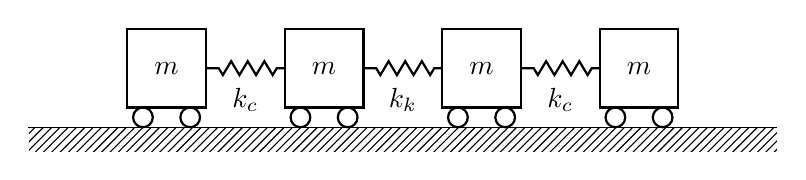
\begin{tikzpicture}
\tikzstyle{spring}=[thick,decorate,decoration={zigzag,pre length=0.1cm,post length=0.1cm,segment length=6}]

\tikzstyle{ground}=[fill,pattern=north east lines,draw=none,minimum width=0.75cm,minimum height=0.3cm]

\node (M) [draw,outer sep=0pt,thick,minimum width=1cm, minimum height=1cm] {$m$};
\node (M2) [draw,outer sep=0pt,thick,minimum width=1cm, minimum height=1cm] at (2,0) {$m$};
\node (M3) [draw,outer sep=0pt,thick,minimum width=1cm, minimum height=1cm] at (4,0) {$m$};
\node (M4) [draw,outer sep=0pt,thick,minimum width=1cm, minimum height=1cm] at (6,0) {$m$};

\node (ground) [ground,anchor=north,xshift=3cm,yshift=-0.25cm,minimum width=9.5cm] at (M.south) {};

\draw (ground.north east) -- (ground.north west);
\draw [thick] (M.south west) ++ (0.2cm,-0.125cm) circle (0.125cm)  (M.south east) ++ (-0.2cm,-0.125cm) circle (0.125cm);
\draw [thick] (M2.south west) ++ (0.2cm,-0.125cm) circle (0.125cm)  (M2.south east) ++ (-0.2cm,-0.125cm) circle (0.125cm);
\draw [thick] (M3.south west) ++ (0.2cm,-0.125cm) circle (0.125cm)  (M3.south east) ++ (-0.2cm,-0.125cm) circle (0.125cm);
\draw [thick] (M4.south west) ++ (0.2cm,-0.125cm) circle (0.125cm)  (M4.south east) ++ (-0.2cm,-0.125cm) circle (0.125cm);

\draw [spring] (M2.180) -- ($(M.north east)!(M.180)!(M.south east)$);
\draw [spring] (M3.180) -- ($(M2.north east)!(M2.180)!(M2.south east)$);
\draw [spring] (M4.180) -- ($(M3.north east)!(M3.180)!(M3.south east)$);

\node at (1,-0.4) {$k_c$};
\node at (3,-0.4) {$k_k$};
\node at (5,-0.4) {$k_c$};

\end{tikzpicture}
\end{center}
\caption{The spring system for $n=2$ subsystems}
\end{figure}

Setting up the general differential equation, assuming no friction, we get
\[
m\frac{d^2}{dt^2} \mathbf{\hat{x}} + \mathbf{K \hat{x}} = 0
\]
where $\mathbf{\hat{x}}$ is a vector containing the relative positions of each mass, $\mathbf{K}$ is the compression matrix shown below:
\[
\begin{pmatrix}
k_c & -k_c &  &  & \dots & 0\\
-k_c & k_c+k_k & -k_k &  & \dots & \\
 & -k_k & k_c+k_k & -k_c & \dots & \vdots \\
 &  & -k_c & k_c + k_k & \dots & \\
\vdots &  &  &  & \ddots & \\
0 &  &  & \dots & -k_c & k_c
\end{pmatrix}
\]

Solving for the eigenvalues of $\mathbf{K}$ symbolically using the following sympy code for the case $n=4$ subsystems (or, 8 masses):


\begin{lstlisting}[language=Python]
from sympy import *
init_printing(use_unicode = True)

w, k, kappa = symbols("w k k'")
firstLine = [k, -k]
evenLine = [-k, k + kappa, -kappa]
oddLine = [-kappa, k+kappa, -k]
lastLine = [-k, k]

def generateMatrix(size):
    mat = []
    mat.append([*firstLine, *[0]*2*(size-1)])
    for i in range((size - 1) * 2):
        if i % 2 is 0:
            mat.append([*[0]*i, *evenLine, *[0]*(2*(size-1)-i - 1)])
        else:
            mat.append([*[0]*i, *oddLine, *[0]*(2*(size - 1) - i - 1)])
    mat.append([*[0]*2*(size - 1), *lastLine])
    return Matrix(mat)

fourCase = generateMatrix(4)
fourEigen = fourCase.eigenvals()
pprint(simplify(fourEigen))
\end{lstlisting}

From running the above code on cases for $n=2,3,4,5,6$, we determined that the eigenvalues follow the following order: First, there will always be two "trivial" eigenvalues that follow for all couplings of the subsystems, even $n=1$:
\[
\lambda = 0,  2k_c
\]
For cases $n>1$, there are the following additional eigenvalues:
\[
\lambda = k_c + k_k \pm \sqrt{k_c^2 + k_k^2 \pm \lambda' k_c k_k}
\]

Where $\lambda'$ was an undetermined variable. Using the code above, we determined the following values of $\lambda'$ for the following values $n$:

\begin{center}
	\begin{tabular}{ c | c}
		$n$ & $\lambda'$ \\
		\hline
		$2$ & $0$ \\
		$3$ & $\pm 1$\\
		$4$ & $0$, $\pm \sqrt{2}$\\
		$5$ & $\frac{\pm 1 \pm \sqrt{5}}{2}$\\
		$6$ & $0$, $\pm 1$, $\pm \sqrt{3}$
	\end{tabular}
\end{center}

As it turns out, $\lambda'$ is actually:
\[
\pm \lambda' = 2\cos\theta
\]
so we can build the following relation:
\begin{center}
	\begin{tabular}{ c | c | c}
		$n$ & $\lambda'$  & $\theta$\\
		\hline
		$2$ & $0$  & $\frac{\pi}{2}$\\
		$3$ & $\pm 1$ & $\frac{\pi}{3}, \frac{2 \pi}{3}$ \\
		$4$ & $0$, $\pm \sqrt{2}$ & $\frac{\pi}{4}, \frac{\pi}{2}, \frac{3\pi}{4}$\\
		$5$ & $\frac{\pm 1 \pm \sqrt{5}}{2}$ & $\frac{\pi}{5}, \frac{2\pi}{5}, \frac{3\pi}{5},\frac{4\pi}{5}$\\
		$6$ & $0$, $\pm 1$, $\pm \sqrt{3}$ &$\frac{\pi}{6}, \frac{\pi}{3}, \frac{\pi}{2}, \frac{2\pi}{3}, \frac{5\pi}{6}$\\
		$\vdots$ & $\vdots$ & $\vdots$\\
		$n$ & $2\cos(a_j)$ & $a_j = \frac{j \pi}{n}$ ; $j \in \mathbb{N} < n$
	\end{tabular}
\end{center}

This allows us to generalize the eigenvalues and combine the "trivial" case with the cases for $n>1$ into:
\[
\lambda = k_c + k_k \pm \sqrt{k_c^2 + k_k^2 - 2 k_c k_k \cos(\theta)}
\]
for the $\theta$s given above. It is thus easy to represent this visually, assuming that $a$ is the greater of $k_c$ and $k_k$ and $b$ is the lesser, with $c$ being the hypotenuse of both these legs:
\begin{figure}[H]
\begin{center}
\begin{tikzpicture}[scale=3]
% place coordinates at the two initial vertices 
\coordinate (a) at (-2,0);
\coordinate (b) at (0,0);

% automatically calculate the third vertex
\path[name path=line 1] (0,0) -- (120:0.85);
\path[name path=line 2] (-2,0) -- (120:0.85);
\path [name intersections={of=line 1 and line 2, by={c}}];
%\path[name path = line 3] (2,0) -- 

% draw the lines
\draw[dashed] (a) -- (c); %hypotenuse
\draw (a) -- (b); %adjacent
\draw (b) -- (c); %opposite

\node at (-1,-0.15) {$a$};
\node at (-0.1, 0.5) {$b$};
\node at (-1.2, .6) {$c$};

% draw the arc clipping a circle against the triangle and place the label
\path[clip] (a) -- (b) -- (c) -- cycle;
\node[circle,draw,minimum size=80pt] at (0,0) (circ) {};
\node[minimum size = 30pt, left] at (circ.140) {$\frac{\pi}{3}$};
\end{tikzpicture}
\end{center}
\caption{eigenvalue for $n=3$ and $\theta = \frac{\pi}{3}$}
\end{figure}

\begin{figure}[H]
\begin{center}
\begin{tikzpicture}[scale=3]
% place coordinates at the two initial vertices 
\coordinate (a) at (-2,0);
\coordinate (b) at (0,0);

% automatically calculate the third vertex
\path[name path=line 1] (0,0) -- (30:0.85);
\path[name path=line 2] (-2,0) -- (30:0.85);
\path [name intersections={of=line 1 and line 2, by={c}}];

% draw the lines
\draw[dashed] (a) -- (c); %hypotenuse
\draw (a) -- (b); %adjacent
\draw (b) -- (c); %opposite

\node at (-1,-0.15) {$a$};
\node at (0.5, 0.15) {$b$};
\node at (-.5, .4) {$c$};

% draw the arc clipping a circle against the triangle and place the label
\path[clip] (a) -- (b) -- (c) -- cycle;
\node[circle,draw,minimum size=20pt] at (0,0) (circ) {};
\node[minimum size = 40pt, left] at (circ.60) {$\frac{2\pi}{3}$};
\end{tikzpicture}
\end{center}
\caption{eigenvalue for $n=3$ and  $\theta = \frac{2\pi}{3}$}
\end{figure}

Because the eigenvalues are dependent on adding or subtracting $c$. The next phase of research involves figuring out how the eigenvalues are geometrically related to these specific triangles. If we take the limits as $n \to \infty$, we would find the following separate bands of eigenvalues forming: The upper band, from $2k_c$ to $2(k_c + k_k)$; and the lower band, from $0$ to $k_c + k_k$. Notably if $k_c = k_k = k$, we get a single band of eigenvalues from $0$ to $4k$. 

We can now go back to the original differential equation:

\[
m \frac{d^2}{dt^2} \mathbf{\hat{x}} = - \mathbf{K \hat{x}}
\]

We can now make the following assumption:
\[
\mathbf{\hat{x}} = \begin{pmatrix}
x_1 e^{i ( \omega t + \phi )} \\
x_2 e^{i ( \omega t + \phi )} \\
x_3 e^{i ( \omega t + \phi )} \\
\vdots \\
x_{2n} e^{i (\omega t + \phi )}
\end{pmatrix}
\]

thus,
\[
-m ( \omega^2 ) \mathbf{\hat{x}} = - \mathbf{K \hat{x}} = - \lambda \mathbf{\hat{x}}
\]
\[
\omega^2 \mathbf{\hat{x}} = \frac{\lambda}{m} \mathbf{\hat{x}}
\]

This is only true for all cases if $\mathbf{\hat{x}}$ is not the zero vector, and thus our normal modes can be constructed as just
\[
\omega = \pm \sqrt{\frac{\lambda}{m}}
\]

Because $\lambda$ encompasses bands from $2k_c$ to $2(k_c + k_k)$ and $0$ to $k_c + k_k$, we can thus define the normal modes of oscillation to have three bands: from $-\sqrt{2( \omega_c^2 + \omega_k^2 )}$ to $- \omega_c \sqrt{2}$, from $-\sqrt{\omega_c^2 + \omega_k^2}$ to $\sqrt{ \omega_c^2 + \omega_k^2}$, and from $\omega_c \sqrt{2}$ to $\sqrt{2 ( \omega_c^2 + \omega_k^2 )}$ where $\omega_{(c,k)}^2 = \frac{k_{(c,k)}}{m}$

\begin{figure}[H]
	\centering
	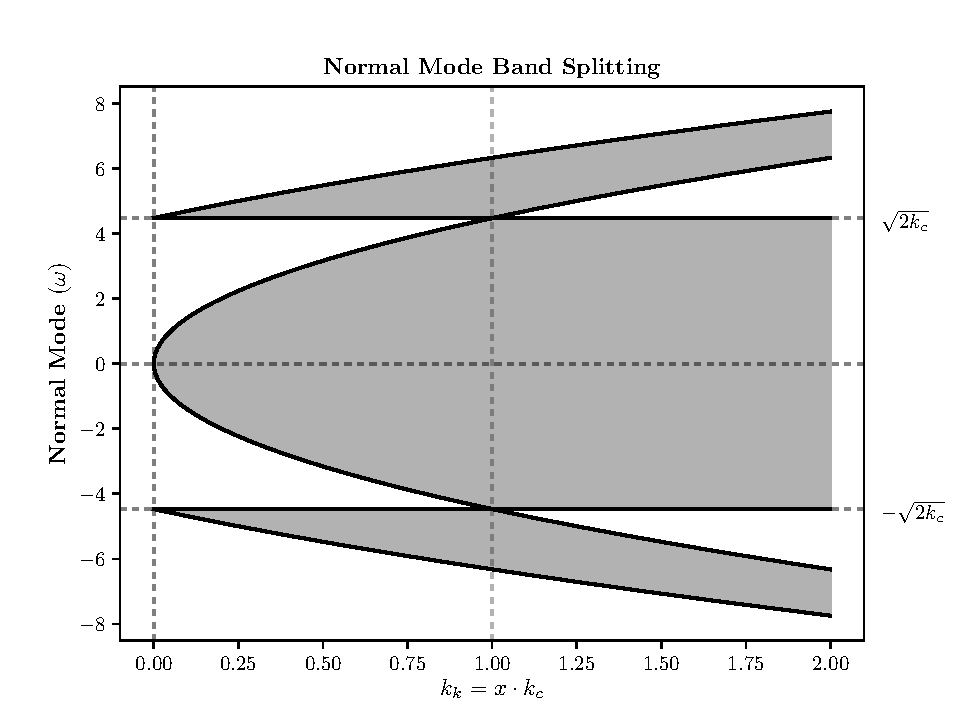
\includegraphics[scale=0.7]{bandSplitting.pdf}
	\caption{Graph for n=500 with $m = 1$}
\end{figure}

\end{document}
